\documentclass{article}
\usepackage[utf8]{inputenc}
\usepackage{graphicx}
    \DeclareGraphicsExtensions{.png, .jpeg}
\usepackage[top=1in, bottom=1in, left=1in, right=1in]{geometry}

\title{CPE 670: Autonomous Mobile Robots \\ Homework $\#1$}
\author{Terence Henriod}
\date{\today}

\begin{document}

\maketitle

\newpage
\begin{enumerate}
\item \textbf{[5 points]} Describe at least 2 differences between the AI and the cybernetics/control theory approaches to robotics. \\

\textbf{Solution:} Cybernetics aims to study and create automatic control systems while AI seeks to create machines that think, reason, and strategize. One difference is that cybernetic systems attempt apply rules to environmental input and use feedback in order to activate or cancel actions that work towards goals, while AI approaches apply those inputs to internal models of the world to search for a solution that will lead to one or more goals. Another difference might be that cybernetic agents tend to be more reactive, while AI agents tend to be more deliberative. Yet another difference would be that cybernetics is more biologically inspired, while AI is more abstract, logical, or philosophical. Others might say that AI is about intelligence by any means, while cybernetics is about descriptive models of systemic organization and feedback. \newline \\


\item \textbf{[5 points]} Explain the difference between the sensory (perceptual) space and the state space of a robot. \\

\textbf{Solution:} The sensory, or perceptual, space is comprised of all possible sensor readings, while the state space is comprised of all possible measures of the robot and its environment. One describes just what a robot can see or become aware of (this is not necessarily real, either), while the other is literally the reality of the robot.

One might say that the perceptual space is a subspace of the state space that grows with the number of sensors used, but this would not be entirely accurate because sensors do not read the true values of reality perfectly. \newline \\


\item \textbf{[10 points]} List at least one advantage and one disadvantage of each of the four robot control paradigms: reactive, deliberative, hybrid, behavior-based. \\

\textbf{Solution:}
    \begin{enumerate}
    \item Reactive - These ``don't think, [just] (re)act." \\
    \textit{Advantage:} Reactive agents can act quickly, and, if designed 
                        properly, can act effectively with little thinking or computation (by referencing built-in or previously learned information). \\
    \textit{Disadvantage:} Reactive agents are incapable of planning out their
                           actions to achieve long-term goals, they can only react to immediate stimuli. \\

    \item Deliberative - ``Think hard, act later" \\
    \textit{Advantage:} Deliberative agents are capable of ``thinking" and
                        planning. This allows them to take actions in ways that are more optimal than systems that do not do this.
                        \\
    \textit{Disadvantage:} These types of agents are slow to react and require
                           a lot of time and resources for computation. They also require accurate models of the world and sensory input to be effective. \\

    \item Hybrid - ``Think and act separately and concurrently" \\
    \textit{Advantage:} Hybrid agents are able to ``have the best of both
                        worlds" in terms of deliberation and reactivity. Hybrids can react for immediate and rapid action, but plan at the same time for long term optimality. \\
    \textit{Disadvantage:} Hybrid agents/robots can be difficult to implement
                        successfully due to issues of concurrency as well as the problem of deciding when to react or when to plan, not to mention the problem of communicating between reactive or deliberate representations of the world (i.e. the ``middle layer"). \\

    \item Behavior-based - ``Think the way you act" \\
    \textit{Advantage:} Behavior-based agents are also capable of being both
                        reactive and deliberative like hybrid ones, but, instead of ``3 layers," these have no middle layer and different \textit{behaviors} (layers) that take inputs from sensory data and other behaviors to determine actions as well as keeping uniform representations and time scales of the world. \\
    \textit{Disadvantage:} Since ``thinking" is performed through a network
                           of behaviors, these can be particularly complex to design effectively. \newline \\
    \end{enumerate}


\item \textbf{[10 points]} The following Braitenberg vehicle has 4 pairs of sensors tuned to different qualities of the environment: light, temperature, oxygen concentration, amount of organic matter. The first pair is connected to the motors with uncrossed excitatory connections, the second pair with crossed excitatory connections, the third and the fourth pairs with inhibitory connections uncrossed and crossed. \\
    \begin{figure}[h!]
    \centering
    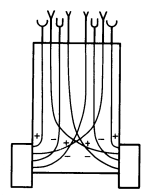
\includegraphics[width = 0.35\textwidth]{Braitenburg_vehicle}
    \caption{The vehicle described in the problem}
    \label{fig:Braitenburg_vehicle}
    \end{figure}
\newline
Describe the behavior of this Braitenberg vehicle, both in terms of direction of movement and in terms of its speed. \\ 

\textbf{Solution:} 
    \begin{enumerate}
    \item Light \\
    Because the connections are excitatory, light will make the vehicle move faster when the light it senses is stronger. However, since the connections are uncrossed, the vehicle will turn away from the light. The result is a photophobic machine that will move away from light quickly at first, then slow down as it sees less light.

    \item Temperature \\
    The connections are again excitatory, meaning the speed of the vehicle will be proportional to the temperature it senses. Because these sensors are crossed, the vehicle will actually move towards higher temperatures. The result is a thermophile that will race towards warmth, and slow down in the presence of cold.

    \item Oxygen \\
    These connections are inhibitory, thus, this vehicle will slow down in the presence of oxygen. Because the connections are uncrossed, the vehicle will end up turning towards oxygen-rich areas. The result is an oxyphile that can only resist going to oxygenated areas. 

    \item Organic Matter \\
    The inhibitory connections make for a robot that slows when organic matter is sensed. The crossing of the connections makes the vehicle turn away from the organic matter should any other stimuli be driving the robot forward. Thus we have an organophobe that needs other stimuli to pull it away from organic matter, but without the other stimuli will only slow its approach towards (turn away from) the organic matter. \newline \\
    \end{enumerate}


\item \textbf{[10 points]} You are to design the sensor capabilities for a new robot for use by fire fighters. The robot is designed to seek out people in a smoke filled building. Keep in mind the following:
    \begin{enumerate}
    \item Visibility is often very limited due to smoke

    \item Heat can be both an attractive force (e.g. human) or repulsive
          (e.g. open flame)

    \item Obstacles may have a wide variety of sound absorption (e.g.
          carpeting or furniture)
    \end{enumerate}

Describe the types of sensors that may be needed and how they will be used. Do not focus on how the robot moves around, just on the sensors it will need to use. \\

\textbf{Solution:} A good design for the robot might use several thermal or infra-red sensors, an IMU (compass/gyroscope), a GPS module, a sonar, and some touch or bend sensors.

The thermal/infra-red sensors would be good candidates for seeking out the people in the building. The robot should use some minimum temperature threshold for finding people in its ``view" and some maximum temperature threshold to differentiate person heat from fire heat.

The IMU and GPS could be used for localization of the robot. GPS might not work so well inside a building, but then again, it might be good enough. The IMU would provide high quality data that would pair well with the use of a map. Of course, fusing the data from these sensors for even better localization would not be a bad idea either. *cough* \emph{Kalman Filter!} *cough*

Finally, the sonar and touch/bend sensors could be used for obstacle avoidance. A sonar is more likely, than say, a lidar unit, to maintain its readings' integrity in the smoky environment. This can give us range finding and help the robot detect landmarks like walls. However, the furniture or other materials and unpredictable sounds in the room may fool the sonar. For this reason, touch or bend sensors (bumpers or whiskers) will also be good to have in the case that some obstacles are just not sensed by the other sensors. The touch/bend sensors will also provide for a reliable, reactive component to the robot's behavior. \\
\end{enumerate}
\end{document}